%%%%%%%%%%%%%%%%%%%%%%%%%%%%%%%%%%%%%%%%%%%%%%%%%%%%%%%%%%%%%%%%%%%%%%%%%%%%%%%%
% Template for USENIX papers.
%
% History:
%
% - TEMPLATE for Usenix papers, specifically to meet requirements of
%   USENIX '05. originally a template for producing IEEE-format
%   articles using LaTeX. written by Matthew Ward, CS Department,
%   Worcester Polytechnic Institute. adapted by David Beazley for his
%   excellent SWIG paper in Proceedings, Tcl 96. turned into a
%   smartass generic template by De Clarke, with thanks to both the
%   above pioneers. Use at your own risk. Complaints to /dev/null.
%   Make it two column with no page numbering, default is 10 point.
%
% - Munged by Fred Douglis <douglis@research.att.com> 10/97 to
%   separate the .sty file from the LaTeX source template, so that
%   people can more easily include the .sty file into an existing
%   document. Also changed to more closely follow the style guidelines
%   as represented by the Word sample file.
%
% - Note that since 2010, USENIX does not require endnotes. If you
%   want foot of page notes, don't include the endnotes package in the
%   usepackage command, below.
% - This version uses the latex2e styles, not the very ancient 2.09
%   stuff.
%
% - Updated July 2018: Text block size changed from 6.5" to 7"
%
% - Updated Dec 2018 for ATC'19:
%
%   * Revised text to pass HotCRP's auto-formatting check, with
%     hotcrp.settings.submission_form.body_font_size=10pt, and
%     hotcrp.settings.submission_form.line_height=12pt
%
%   * Switched from \endnote-s to \footnote-s to match Usenix's policy.
%
%   * \section* => \begin{abstract} ... \end{abstract}
%
%   * Make template self-contained in terms of bibtex entires, to allow
%     this file to be compiled. (And changing refs style to 'plain'.)
%
%   * Make template self-contained in terms of figures, to
%     allow this file to be compiled. 
%
%   * Added packages for hyperref, embedding fonts, and improving
%     appearance.
%   
%   * Removed outdated text.
%
%%%%%%%%%%%%%%%%%%%%%%%%%%%%%%%%%%%%%%%%%%%%%%%%%%%%%%%%%%%%%%%%%%%%%%%%%%%%%%%%

\documentclass[letterpaper,twocolumn,10pt]{article}
\usepackage{usenix-2020-09}

% to be able to draw some self-contained figs
\usepackage{tikz}
\usepackage{amsmath}

% inlined bib file
\usepackage{filecontents}

%-------------------------------------------------------------------------------
\begin{filecontents}{\jobname.bib}
%-------------------------------------------------------------------------------
@Book{arpachiDusseau18:osbook,
  author =       {Arpaci-Dusseau, Remzi H. and Arpaci-Dusseau Andrea C.},
  title =        {Operating Systems: Three Easy Pieces},
  publisher =    {Arpaci-Dusseau Books, LLC},
  year =         2015,
  edition =      {1.00},
  note =         {\url{http://pages.cs.wisc.edu/~remzi/OSTEP/}}
}
@InProceedings{waldspurger02,
  author =       {Waldspurger, Carl A.},
  title =        {Memory resource management in {VMware ESX} server},
  booktitle =    {USENIX Symposium on Operating System Design and
                  Implementation (OSDI)},
  year =         2002,
  pages =        {181--194},
  note =         {\url{https://www.usenix.org/legacy/event/osdi02/tech/waldspurger/waldspurger.pdf}}}
\end{filecontents}

%-------------------------------------------------------------------------------
\begin{document}
%-------------------------------------------------------------------------------

%don't want date printed
\date{}

% make title bold and 14 pt font (Latex default is non-bold, 16 pt)
\title{\Large \bf INFO5995 Cybersecurity Assignment 1\\
  AI-Assisted Cryptographic Vulnerability Discovery}

%for single author (just remove % characters)
\author{
{\rm Handong Ding}\\
the University of Sydney
\and
{\rm Student ID:}\\
% copy the following lines to add more authors
% \and
% {\rm Name}\\
%Name Institution
} % end author

\maketitle

%-------------------------------------------------------------------------------
\begin{abstract}
%-------------------------------------------------------------------------------

This report presents a security audit of the com.example.mastg\_test0016 Android application. The objective was to identify vulnerabilities related to data persistence and cryptographic randomness using AI-assisted static analysis. Through decompilation, we discovered that the application stores sensitive user credentials in plaintext and utilizes a predictable pseudo-random number generator (PRNG) for security-sensitive values. These flaws expose users to credential theft and session hijacking. We recommend implementing hardware-backed encryption and cryptographically secure PRNGs to mitigate these risks.

\end{abstract}


%-------------------------------------------------------------------------------
\section{Introduction}
%-------------------------------------------------------------------------------

Goal: The primary goal is to assess how the application handles sensitive assets and whether its cryptographic implementations meet industry standards.

APK \& Decompilation: An APK (Android Package) is the distribution file format for Android, containing compiled Dalvik bytecode (.dex), resources, and metadata. Decompilation is essential for auditing because it translates the machine-readable binary back into human-readable Java code. This process allows auditors to inspect internal logic, such as hardcoded secrets and flawed algorithms, which are invisible during standard app usage.

App Summary: The application is a user management utility that facilitates new user registration and authentication. Users register by entering a username and password, which the app saves to a local file. After a successful login, the app navigates to a profile screen and utilizes a random number generator to handle session-related data or identifiers.

%-------------------------------------------------------------------------------
\section{System and Threat Model}
%-------------------------------------------------------------------------------

% Footnotes should be places after punctuation characters, without any
% spaces between said characters and footnotes, like so.%
% \footnote{Remember that USENIX format stopped using endnotes and is
%   now using regular footnotes.} And some embedded literal code may
% look as follows.

Core Assumptions \& Attacker Goals:
We assume the developer believes that the application’s private storage is inaccessible to other apps and that java.util.Random provides sufficient entropy. The Attacker’s Goal is to bypass authentication or impersonate legitimate users by either stealing stored credentials or predicting future session codes.

Value Generation \& Unsuitability:
In MainActivity.java, the security-sensitive random value is generated via new Random().nextInt(100). This method is unsuitable for a security role (such as a session token or OTP) because it is a linear congruential generator (LCG). It is deterministic and has a small state space (48-bit seed), making it mathematically predictable.

Attacker Model \& Capabilities:
We define a Rooted-Device User or a Malicious Side-loaded App as the primary threat.

Capabilities: The attacker can read the application's private files in /data/data/, monitor system logs (Logcat), and use computational tools to reverse-engineer PRNG states.

Step-by-Step Attack Scenario (Impersonation):

Observation: The attacker observes several outputs of the randomNumberGenerator via Logcat.

State Reconstruction: Using the observed values, the attacker reconstructs the internal state of the 48-bit PRNG seed.

Prediction: The attacker calculates the next value the app will generate for a victim's session.

Bypass: The attacker injects the predicted value into the authentication flow, successfully impersonating the victim.

\begin{figure}[htbp]
    \centering
    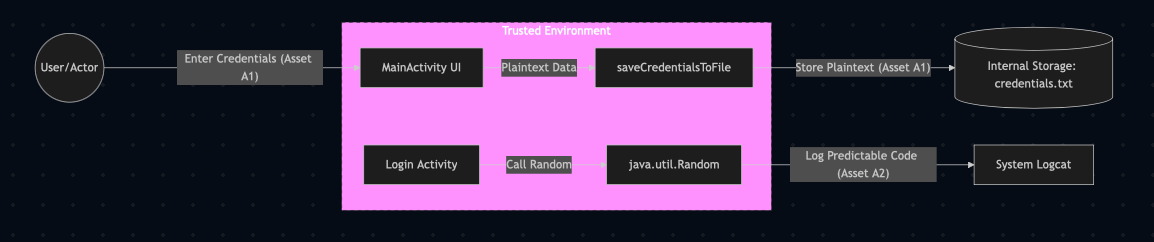
\includegraphics[width=\columnwidth]{DFD}
    \caption{Data Flow Diagram}
    \label{fig:my_image}
\end{figure}

% \begin{verbatim}
% int main(int argc, char *argv[]) 
% {
%     return 0;
% }
% \end{verbatim}

% Now we're going to cite somebody. Watch for the cite tag. Here it
% comes. Arpachi-Dusseau and Arpachi-Dusseau co-authored an excellent OS
% book, which is also really funny~\cite{arpachiDusseau18:osbook}, and
% Waldspurger got into the SIGOPS hall-of-fame due to his seminal paper
% about resource management in the ESX hypervisor~\cite{waldspurger02}.

% The tilde character (\~{}) in the tex source means a non-breaking
% space. This way, your reference will always be attached to the word
% that preceded it, instead of going to the next line.

% And the 'cite' package sorts your citations by their numerical order
% of the corresponding references at the end of the paper, ridding you
% from the need to notice that, e.g, ``Waldspurger'' appears after
% ``Arpachi-Dusseau'' when sorting references
% alphabetically~\cite{waldspurger02,arpachiDusseau18:osbook}. 

% It'd be nice and thoughtful of you to include a suitable link in each
% and every bibtex entry that you use in your submission, to allow
% reviewers (and other readers) to easily get to the cited work, as is
% done in all entries found in the References section of this document.

% Now we're going take a look at Section~\ref{sec:figs}, but not before
% observing that refs to sections and citations and such are colored and
% clickable in the PDF because of the packages we've included.

%-------------------------------------------------------------------------------
\section{Discovery Methodology}
\label{sec:figs}
%-------------------------------------------------------------------------------

The vulnerability discovery was conducted using JADX-GUI for static analysis.

Tooling: JADX-GUI allowed for the reconstruction of the sources directory from the APK.

AI Assistance: After locating the MainActivity and saveCredentialsToFile methods, the code was analyzed with the assistance of Gemini 3 Flash.

Process: I prompted the AI to "identify cryptographic misuse and insecure data storage patterns." The AI successfully highlighted that Random() is not a CSPRNG and flagged the lack of encryption in the file writing logic.

%---------------------------
% \begin{figure}
% \begin{center}
% \begin{tikzpicture}
%   \draw[thin,gray!40] (-2,-2) grid (2,2);
%   \draw[<->] (-2,0)--(2,0) node[right]{$x$};
%   \draw[<->] (0,-2)--(0,2) node[above]{$y$};
%   \draw[line width=2pt,blue,-stealth](0,0)--(1,1)
%         node[anchor=south west]{$\boldsymbol{u}$};
%   \draw[line width=2pt,red,-stealth](0,0)--(-1,-1)
%         node[anchor=north east]{$\boldsymbol{-u}$};
% \end{tikzpicture}
% \end{center}
% \caption{\label{fig:vectors} Text size inside figure should be as big as
%   caption's text. Text size inside figure should be as big as
%   caption's text. Text size inside figure should be as big as
%   caption's text. Text size inside figure should be as big as
%   caption's text. Text size inside figure should be as big as
%   caption's text. }
% \end{figure}
%% %---------------------------


% Here's a typical reference to a floating figure:
% Figure~\ref{fig:vectors}. Floats should usually be placed where latex
% wants then. Figure\ref{fig:vectors} is centered, and has a caption
% that instructs you to make sure that the size of the text within the
% figures that you use is as big as (or bigger than) the size of the
% text in the caption of the figures. Please do. Really.

% In our case, we've explicitly drawn the figure inlined in latex, to
% allow this tex file to cleanly compile. But usually, your figures will
% reside in some file.pdf, and you'd include them in your document
% with, say, \textbackslash{}includegraphics.

% Lists are sometimes quite handy. If you want to itemize things, feel
% free:

% \begin{description}
  
% \item[fread] a function that reads from a \texttt{stream} into the
%   array \texttt{ptr} at most \texttt{nobj} objects of size
%   \texttt{size}, returning returns the number of objects read.

% \item[Fred] a person's name, e.g., there once was a dude named Fred
%   who separated usenix.sty from this file to allow for easy
%   inclusion.
% \end{description}

% \noindent
% The noindent at the start of this paragraph in its tex version makes
% it clear that it's a continuation of the preceding paragraph, as
% opposed to a new paragraph in its own right.


% \subsection{LaTeX-ing Your TeX File}
% %-----------------------------------

% People often use \texttt{pdflatex} these days for creating pdf-s from
% tex files via the shell. And \texttt{bibtex}, of course. Works for us.

%-------------------------------------------------------------------------------
\section{Vulnerability Details}
%-------------------------------------------------------------------------------

% The USENIX latex style is old and very tired, which is why
% there's no \textbackslash{}acks command for you to use when
% acknowledging. Sorry.

Code Location:

MainActivity.java: randomNumberGenerator() (Line 16)

MainActivity.java: saveCredentialsToFile() (Line 50)

Risk Assessment:

CWE-312 (Plaintext Storage): Violates Confidentiality. Credentials are saved to credentials.txt without any transformation.

CWE-338 (Weak PRNG): Violates Integrity. The generator pattern java.util.Random is entirely unsuitable for security-sensitive values because its output is predictable.

Core Vulnerability:
The Cryptographically Weak PRNG usage is selected as the core vulnerability. While the plaintext storage is a severe flaw, the weak PRNG directly compromises the authentication behavior of the app. Per Week 4 theory, a secure PRG must satisfy the "next-bit test," where no attacker can predict s 
n+1
​	
  with probability >0.5. java.util.Random fails this test fundamentally.

%-------------------------------------------------------------------------------
\section{Concrete Fix \& Mitigation}
%-------------------------------------------------------------------------------

The Fix:

Randomness: Replace java.util.Random with java.security.SecureRandom.

Storage: Replace openFileOutput with EncryptedSharedPreferences from the Android Jetpack Security library.

Why it works:
SecureRandom is a CSPRNG that uses non-deterministic entropy from the OS (e.g., /dev/urandom). Mathematically, it ensures that the output is computationally indistinguishable from a true random sequence. EncryptedSharedPreferences ensures that even if an attacker with root access steals the credentials.txt file, the data is encrypted using keys protected by the Android Keystore System, rendering the stolen data useless.

%-------------------------------------------------------------------------------
\bibliographystyle{plain}
\bibliography{\jobname}

%%%%%%%%%%%%%%%%%%%%%%%%%%%%%%%%%%%%%%%%%%%%%%%%%%%%%%%%%%%%%%%%%%%%%%%%%%%%%%%%
\end{document}
%%%%%%%%%%%%%%%%%%%%%%%%%%%%%%%%%%%%%%%%%%%%%%%%%%%%%%%%%%%%%%%%%%%%%%%%%%%%%%%%

%%  LocalWords:  endnotes includegraphics fread ptr nobj noindent
%%  LocalWords:  pdflatex acks